\subsubsection{Components of usability}
Based on Nielsen 2012 (https://medium.com/@iizzathisharah/the-five-usability-components-by-jakob-nielsen-detailed-insights-and-examples-90695af5ffb6)

\begin{itemize}
    \item learnability
    \item efficiency
    \item memorabiliy
    \item errors
    \item satisfaction
\end{itemize}

\newpage
\subsubsection{Usability testing}
Magpie has remedied the first challenge of fragmented information on
amenities, and through this user evaluation, we hope to address the second challenge
which is making the access to this information easy, quick \& accessible.\\\\

The goal of the user evaluation is to gain feedback from real users, learn if
Magpie works as expected and assess how user-friendly it is. We will be using 2
main methods to collect both qualitative data through open-ended questions, and
quantitative data from multiple choice questions from which we will derive
insights to improve the Magpie user experience.\\\\

Our approach was as follows:
%user evaluation approach
\begin{enumerate}
    \item Round up users from the market research + seek out others
    \item Conduct online sessions to discuss Magpie, explore the features, gather feedback,
    \item Fill out satisfaction survey
    \item Synthesize notes from sessions and summarize points to improve
    \item Iteratively implement/improve features
\end{enumerate}

These sessions followed an uncontrolled usability testing approach where we let the users freely roam the application while observing their behaviour interacting with each element, guide them when they were stuck and initiate discussion on the topic of amenities, use cases for the application and feedback on features to improve.\\\\
We used a table with a list of general tasks that the user to quantitatively evaluate each feature on its ease of completion, intuitiveness and action. The list of general tasks increased as the test sessions went on because we were iteratively adding new features.\\\\
The difficulty of the task is related to if they were able to complete it and how much they struggled during it. The status of a task can either be "complete", "pass", or "fail" where "complete" is attributed when the user does the task on their own, "pass" is attributed when the user was able to complete the task but with our help, and "fail" when the user were not able to do the task even with our help. \\\\
In addition, the user's behavior is observed to give us indications on their thought process and their intuition going through a map based application like Magpie.\\\\
We also had a short satisfaction survey to quantitatively evaluate each user test session. This helps us see if Magpie improves as the test sessions go on. Each session will be presented chronologically starting with Paul.
%figure for satisfaction survey
\begin{figure}
    \centering
    \fbox{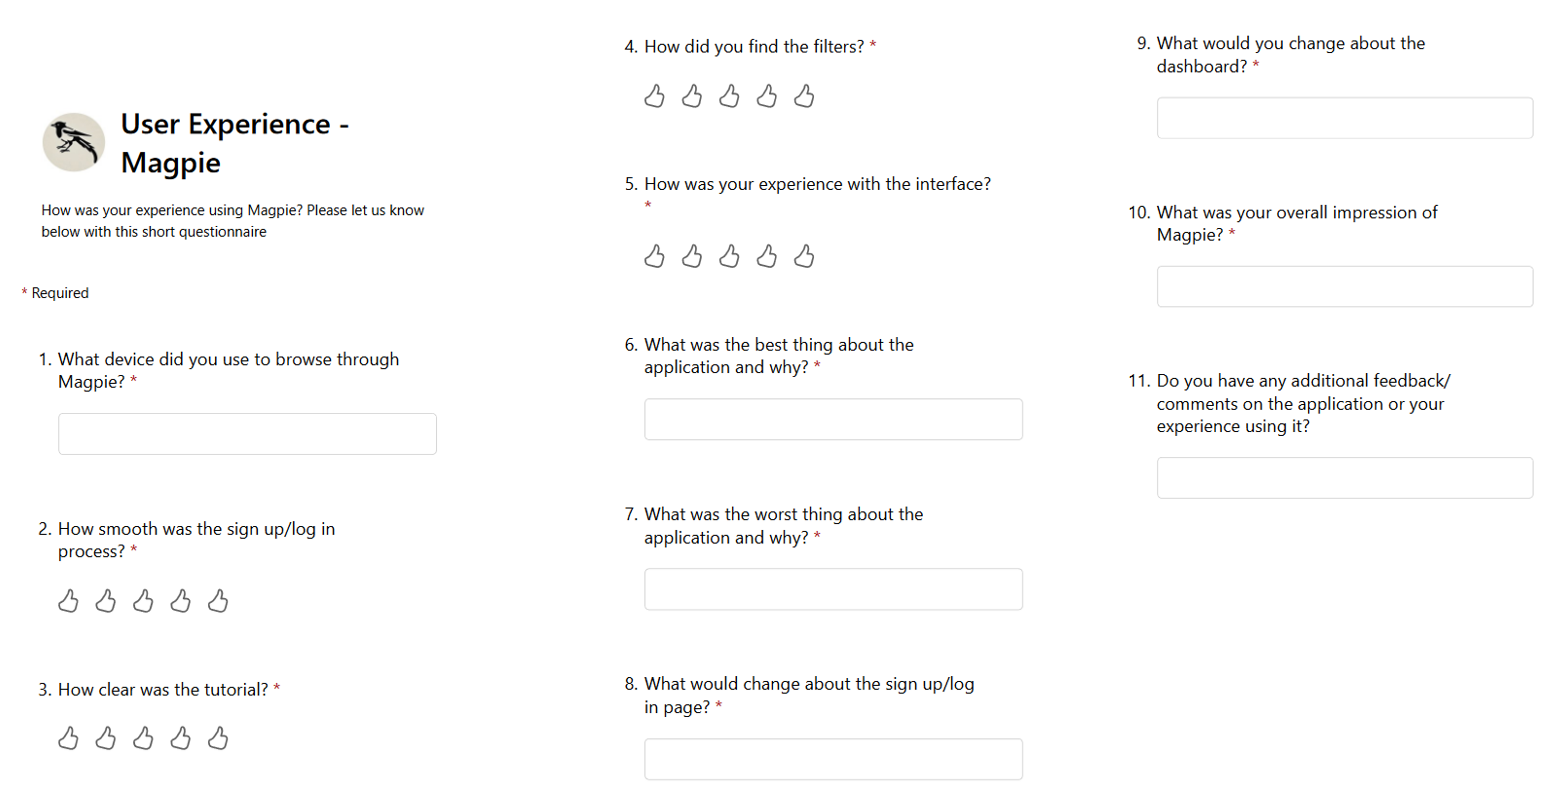
\includegraphics[width=0.8\textwidth]{images/user-satisfaction-survey.png}}
    \caption{User Evaluation - Satisfaction survey questions}
\end{figure}

\newpage
\subsubsection{User 1 - Paul}
Our first test session was with Paul, a student in technological undergraduate degree. They are classified as a general user, not one we have identified as our target. They left their contact email in the market research survey.\\
We initially wanted this to be a controlled test session by giving him specific tasks, but found that challenging as he intuitively went on to explore the application on his own.
%table of Paul's general tasks
\begin{table}[h!]
    \centering
    \caption{Usability testing Tasks - Paul}
    \begin{tabular}{|p{0.4\textwidth}|p{0.1\textwidth}|p{0.1\textwidth}|p{0.1\textwidth}|p{0.1\textwidth}|}
        \hline
        \textbf{Task}                                 & \textbf{Status} & \textbf{Time taken} & \textbf{Difficulty} & \textbf{Errors}    \\
        \hline
        Load Magpie application                       & Complete        & 20s                 & 1                   & N/A                \\
        \hline
        Sign up                                       & Complete        & 42s                 & 1                   & N/A                \\
        \hline
        Complete tutorial                             & Complete        & 60s                 & 1                   & N/A                \\
        \hline
        Place cursor on map and adjust radius to 250m & Fail            & Skipped             & Skipped             & Skipped            \\
        \hline
        Zoom in to road name level                    & Complete        & 5s                  & 1                   & N/A                \\
        \hline
        Place cursor on another area                  & Complete        & 5s                  & 1                   & N/A                \\
        \hline
        Zoom out to see full radius                   & Fail            & Skipped             & Skipped             & Skipped            \\
        \hline
        Filter to only view "Parking meter" data      & Pass            & 120s                & 3                   & Required help      \\
        \hline
        Filter to toggle off all amenities            & Pass            & 37s                 & 3                   & Required help      \\
        \hline
        Go through tutorial and exit at Step 3        & Pass            & 30s                 & 3                   & Couldn't find icon \\
        \hline
        Log out                                       & Complete        & 20s                 & 2                   & N/A                \\
        \hline
    \end{tabular}
\end{table}
\textbf{Main takeaways from Paul's session: }the map display and the amenity data displayed is "excellent", they would find it useful for local areas of the city. One aspect they advise we improve on is to make the choice of amenities more intuitive. This is further supported by his behaviour trying to click on the icon and subsequent amenity title on the dashboard to toggle it on and off, as well as the difficulties he encountered as shown in the general task table.\\
Another point to improve on is to make the profile and tutorial icons more visible, demonstrated by the time it took him to find them and complete the general tasks.\\\\
\textbf{Score from survey: }
%paul survey score
\begin{figure}
    \centering
    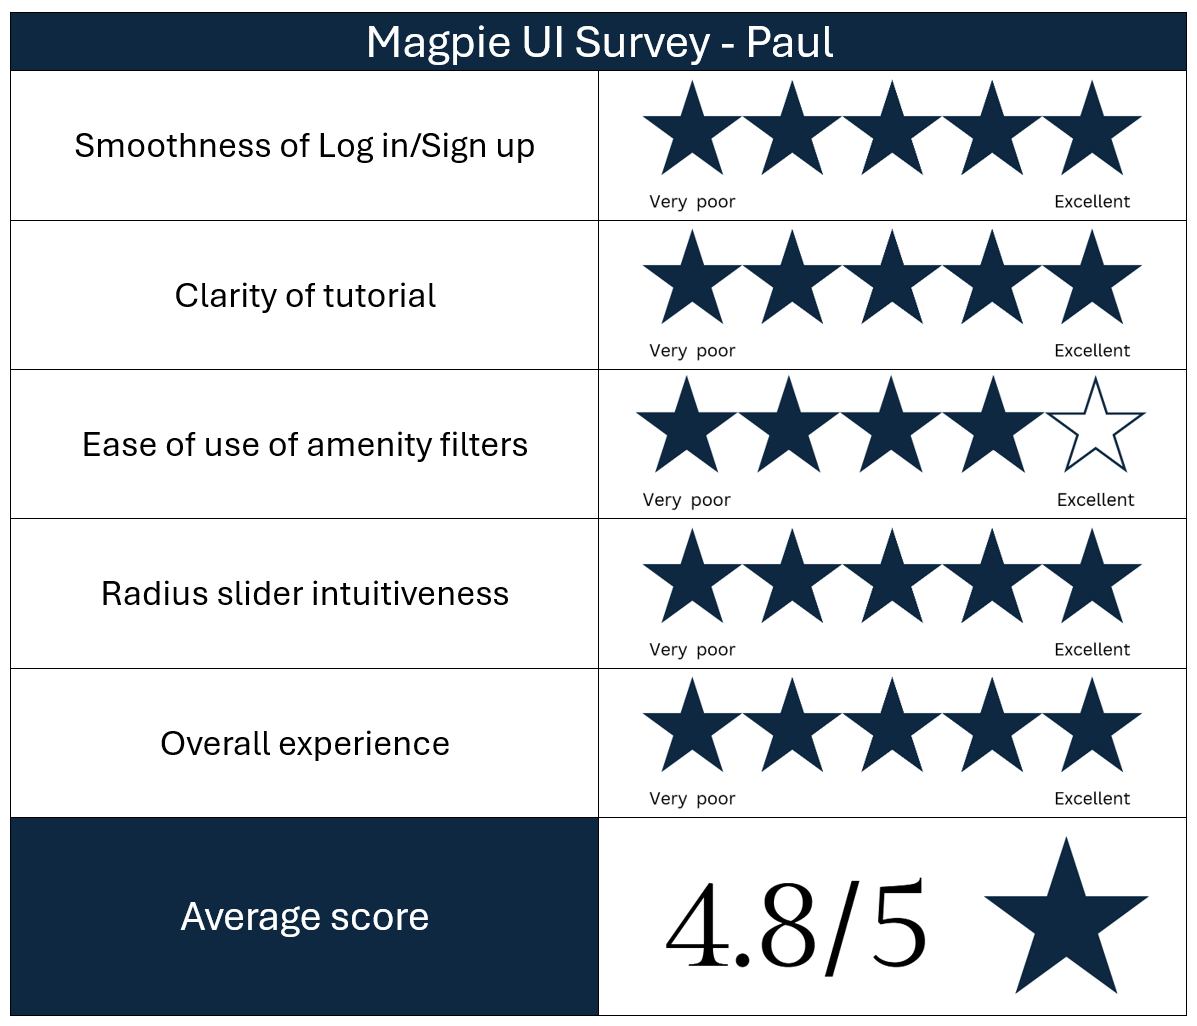
\includegraphics[width=0.8\textwidth]{images/survey-paul.png}
    \caption{User Evaluation - UI Score Paul}
\end{figure}

\newpage
\subsubsection{User 2 - Livia}
Our second test session was with Livia, another student in a technological undergraduate degree. They are also identified as a casual user who also left their contact in the market research survey.\\\\
This session also started out as a controlled test with a defined set of tasks, but just like Paul, Livia went on to explore the application skipping the tasks.\\\\
%table of Livias's general tasks
\begin{table}[h!]
    \centering
    \caption{Usability testing Tasks - Livia}
    \begin{tabular}{|p{0.4\textwidth}|p{0.1\textwidth}|p{0.1\textwidth}|p{0.1\textwidth}|p{0.1\textwidth}|}
        \hline
        \textbf{Task}                                 & \textbf{Status} & \textbf{Time taken} & \textbf{Difficulty} & \textbf{Errors} \\
        \hline
        Load Magpie application                       & Complete        & 5s                  & 1                   & N/A             \\
        \hline
        Sign up                                       & Complete        & 16s                 & 1                   & N/A             \\
        \hline
        Complete tutorial                             & Complete        & 44s                 & 1                   & N/A             \\
        \hline
        Place cursor on map and adjust radius to 250m & Complete        & 6s                  & 1                   & N/A             \\
        \hline
        Zoom in to road name level                    & Complete        & 8s                  & 1                   & N/A             \\
        \hline
        Place cursor on another area                  & Fail            & Skipped             & Skipped             & Skipped         \\
        \hline
        Zoom out to see full radius                   & Fail            & Skipped             & Skipped             & Skipped         \\
        \hline
        Filter to only view "Parking meter" data      & Fail            & Skipped             & Skipped             & Skipped         \\
        \hline
        Filter to toggle off all amenities            & Complete        & 18s                 & 1                   & N/A             \\
        \hline
        Go through tutorial and exit at Step 3        & Complete        & 24s                 & 2                   & N/A             \\
        \hline
        Log out                                       & Complete        & 20s                 & 2                   & N/A             \\
        \hline
    \end{tabular}
\end{table}
\textbf{Main takeaways from Livia's session: }very interesting project, useful and great; overall a very clear website. Biggest point of discontent for Livia was the tutorial, they let us know they has dyslexia and the tutorial could've been worded more effectively to cater to them and others with learning/visual impediments. In addition, they tried to interact with the locked elements during the tutorial, suggesting intuition to put in practice what they are reading to validate the information absorbed.\\\\
They also suggested adding more amenities such as public transports stops, scooter stands and student hubs. They liked how it was easier to understand the information visually compared to Google maps or Apple maps.\\\\
\textbf{Score from survey: }
%livia survey score
\begin{figure}
    \centering
    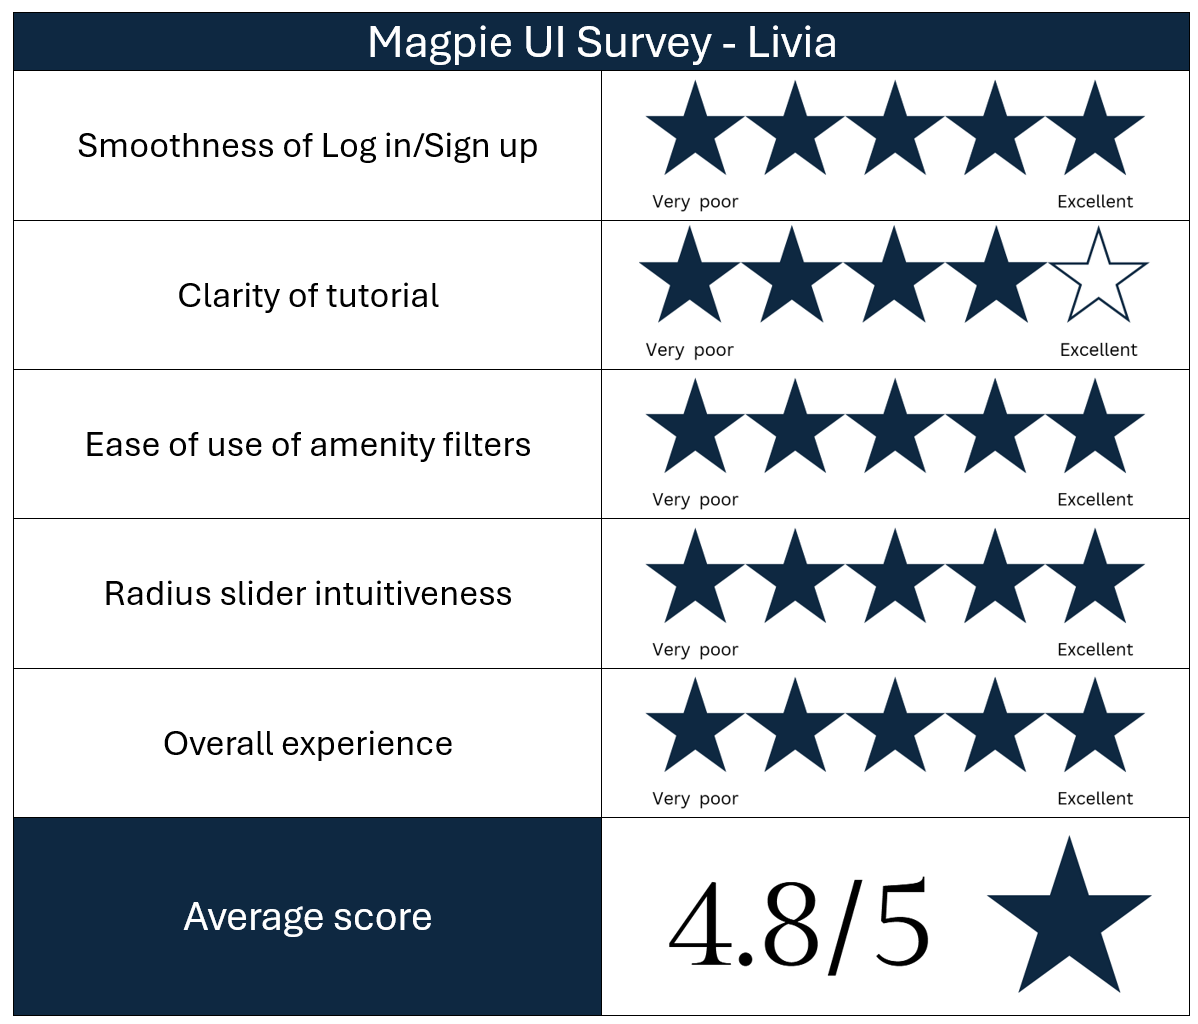
\includegraphics[width=0.8\textwidth]{images/survey-livia.png}
    \caption{User Evaluation - UI Score Livia}
\end{figure}

\newpage
\subsubsection{User 3 - Ben}
Our third test session was with Ben, another student in a technological post-graduate degree. They are also identified as a casual user who also left their contact in the market research survey.\\\\
Starting this session, we took a more uncontrolled approach and let the users free roam the application without giving them specific tasks to complete. We guided them in the beginning and initiated certain discussions but overall let the users take the reign and think aloud during their exploration process.\\\\
%table of Ben's general tasks
\begin{table}[h!]
    \centering
    \caption{Usability testing Tasks - Ben}
    \begin{tabular}{|p{0.4\textwidth}|p{0.1\textwidth}|p{0.1\textwidth}|p{0.1\textwidth}|p{0.1\textwidth}|}
        \hline
        \textbf{Task}                 & \textbf{Status} & \textbf{Difficulty} & \textbf{Errors} \\
        \hline
        Load Magpie application       & Complete        & 1                   & N/A             \\
        \hline
        Sign up                       & Complete        & 1                   & N/A             \\
        \hline
        Log in                        & Complete        & 1                   & N/A             \\
        \hline
        Complete tutorial             & Complete        & 1                   & N/A             \\
        \hline
        Place cursor on map           & Complete        & 1                   & N/A             \\
        \hline
        Zoom in and out               & Complete        & 1                   & N/A             \\
        \hline
        Hold map and navigate         & Complete        & 1                   & N/A             \\
        \hline
        Adjust radius big/small       & Complete        & 1                   & N/A             \\
        \hline
        Clear marker \& radius        & Skipped         & Skipped             & Skipped         \\
        \hline
        Deselect all amenities        & Complete        & 1                   & N/A             \\
        \hline
        Select one or more amenities  & Complete        & 1                   & N/A             \\
        \hline
        Find tutorial and exit midway & Skipped         & Skipped             & Skipped         \\
        \hline
        Log out                       & Complete        & 1                   & N/A             \\
        \hline
    \end{tabular}
\end{table}
\textbf{Main takeaways from Ben's session: }the application does exactly what we described it to do- a GIS application to give a at a glance of amenities in Dublin. The overall impression is that it's a very helpful application, easy to use and effective.\\
Points to improve are the loading times for the amenity points, perhaps  directly being logged in after sign up to avoid repetitive steps, make the profile and tutorial icons more visible as they blend into the map, remove mac keyboard icons from the profile bubble, and if possible add more information on each amenity perhaps with tooltips, or add more amenity data like public transportation.\\\\
\textbf{Score from survey: }
%ben survey score
\begin{figure}
    \centering
    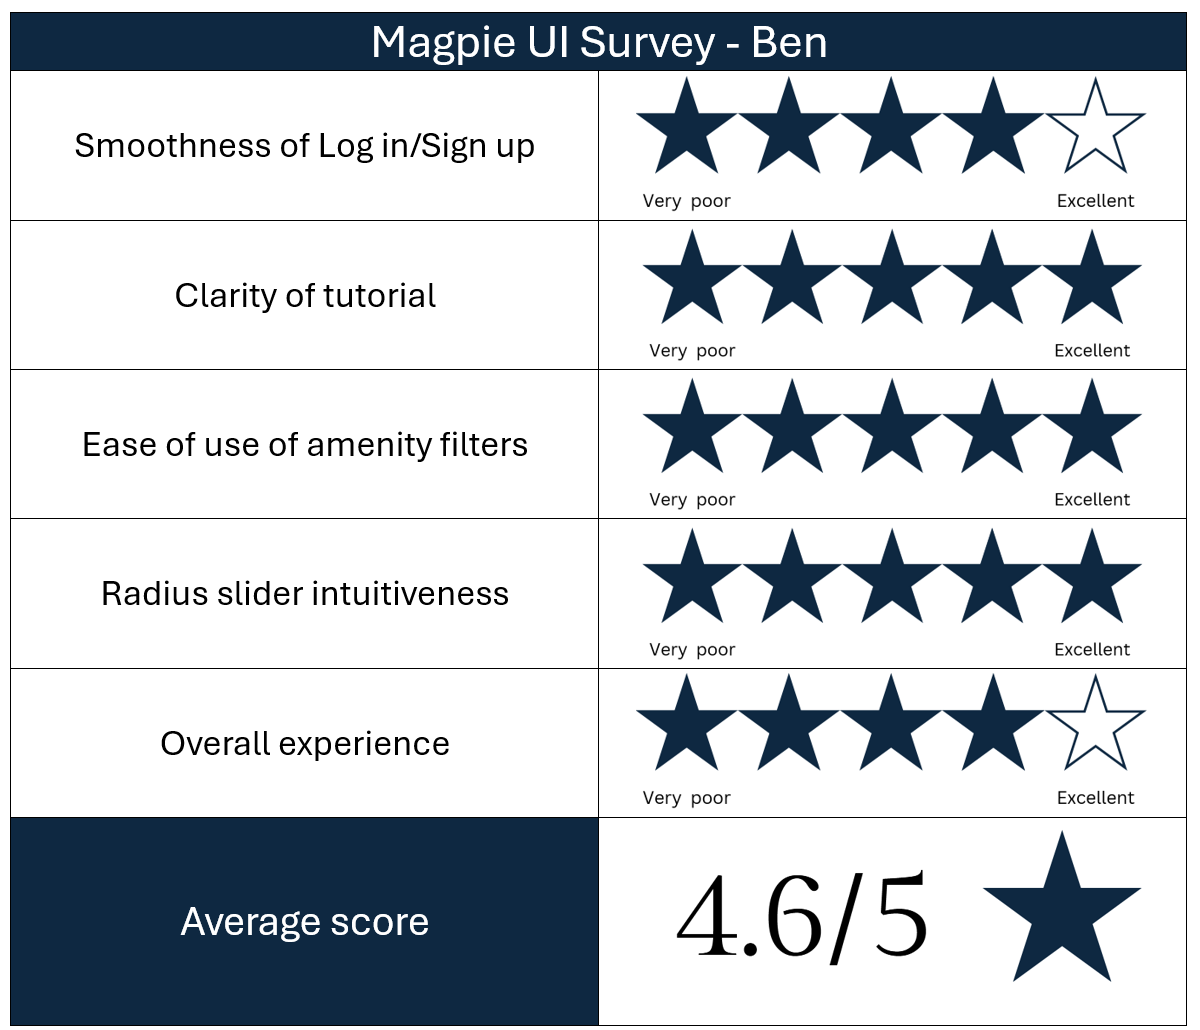
\includegraphics[width=0.8\textwidth]{images/survey-ben.png}
    \caption{User Evaluation - UI Score Ben}
\end{figure}

\newpage
\subsubsection{User 4 - Jakub}
Casual user Jakub

\newpage
\subsubsection{User 5 - Brendan}
Casual user Brendan

\newpage
\subsubsection{User 6 - Anonymous}
Casual user Maira

\newpage
\subsubsection{User 7 - Bryan Boyle}
Professional user Bryan

\newpage
\subsubsection{User 8 - Anonymous}
Professional user Sarah

\newpage
\subsubsection{User 9 - Anonymous}
Professional user Odran
